% Shared standalone design for the editable figure reconstructions.
\documentclass[tikz,border=5pt,10pt]{standalone}
\usepackage[T1]{fontenc}
\usepackage[utf8]{inputenc}
\usepackage{newpxtext,newpxmath}
\usepackage[scaled=.94]{sourcesanspro}
\usepackage{pgfplots}
\pgfplotsset{compat=1.18}
\usetikzlibrary{arrows.meta,calc,positioning,decorations.pathreplacing,
  decorations.markings,patterns,matrix,shapes.geometric,fit,backgrounds,
  intersections,angles,quotes}
\definecolor{ink}{HTML}{203746}
\definecolor{accent}{HTML}{146C78}
\definecolor{muted}{HTML}{667780}
\definecolor{signalred}{HTML}{B94B44}
\color{ink}
\tikzset{>=Latex,line width=.8pt,
  every node/.style={font=\small},
  axis/.style={->,draw=muted,line width=.5pt},
  guide/.style={draw=muted,dashed,line width=.45pt},
  curve/.style={draw=accent,line width=1pt},
  marker/.style={circle,fill=accent,inner sep=1.5pt},
  labelbox/.style={fill=white,inner sep=2pt}}

\begin{document}
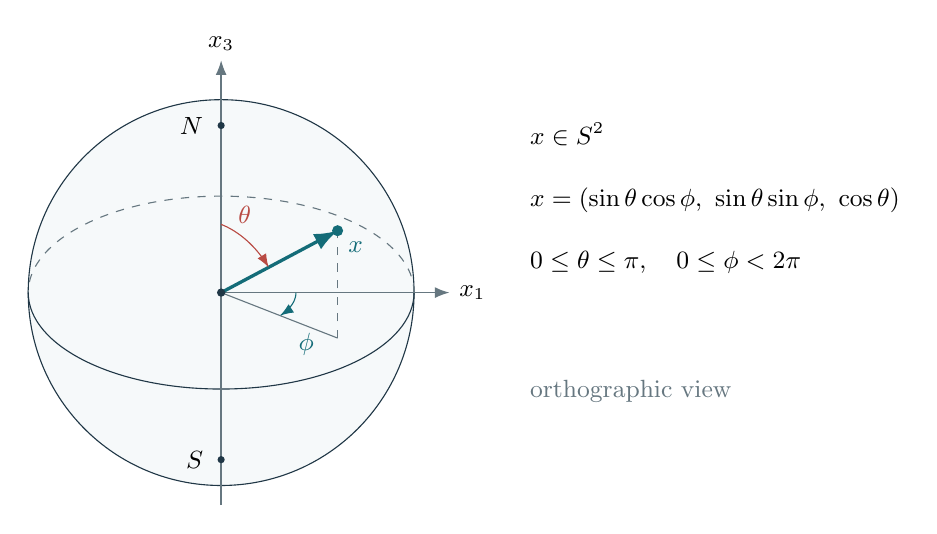
\begin{tikzpicture}[x=1cm,y=1cm]
% Orthographic projection P(a,b,c)=(a,-b sin(e)+c cos(e)), e=30 degrees.
% The projection has orthonormal rows, so the sphere silhouette is a circle.
\def\Radius{2.45}\def\Elevation{30}\def\Theta{50}\def\Phi{38}
\pgfmathsetmacro\EquatorHeight{\Radius*sin(\Elevation)}
\pgfmathsetmacro\PoleHeight{\Radius*cos(\Elevation)}
\coordinate (p) at ({\Radius*sin(\Theta)*cos(\Phi)},{-\Radius*sin(\Theta)*sin(\Phi)*sin(\Elevation)});
\coordinate (x) at ({\Radius*sin(\Theta)*cos(\Phi)},{\Radius*(-sin(\Theta)*sin(\Phi)*sin(\Elevation)+cos(\Theta)*cos(\Elevation))});
\fill[accent!4] (0,0) circle(\Radius);
\draw[ink] (0,0) circle(\Radius);
\draw[muted,dashed] (\Radius,0) arc[start angle=0,end angle=180,x radius=\Radius,y radius=\EquatorHeight];
\draw[ink] (-\Radius,0) arc[start angle=180,end angle=360,x radius=\Radius,y radius=\EquatorHeight];
\draw[axis] (0,-2.7)--(0,2.95) node[above] {$x_3$};
\fill[ink] (0,\PoleHeight) circle(1.3pt) (0,-\PoleHeight) circle(1.3pt);
\node[left=3pt] at (0,\PoleHeight) {$N$};\node[left=3pt] at (0,-\PoleHeight) {$S$};
\draw[axis] (0,0)--(2.9,0) node[right] {$x_1$};
\draw[guide] (p)--(x);\draw[muted] (0,0)--(p);
\draw[->,accent,line width=1.2pt] (0,0)--(x) node[below right] {$x$};
% Project the actual colatitude arc in the meridian of x.
\draw[->,signalred,domain=0:\Theta,samples=51] plot ({sin(\x)*cos(\Phi)},{-sin(\x)*sin(\Phi)*sin(\Elevation)+cos(\x)*cos(\Elevation)});
\node[signalred] at (.30,.99) {$\theta$};
% Project the actual azimuth arc in the equatorial plane.
\draw[->,accent,domain=0:\Phi,samples=41] plot ({.95*cos(\x)},{-.95*sin(\x)*sin(\Elevation)});
\node[accent] at (1.08,-.66) {$\phi$};
\fill[ink] (0,0) circle(1.5pt);\fill[accent] (x) circle(2pt);
\node[anchor=west,align=left] at (3.8,1.2) {$x\in\mathbb S^2$\\[4mm]$x=(\sin\theta\cos\phi,\ \sin\theta\sin\phi,\ \cos\theta)$\\[4mm]$0\le\theta\le\pi,\quad 0\le\phi<2\pi$};
\node[muted,anchor=west] at (3.8,-1.25) {orthographic view};
\end{tikzpicture}
\end{document}
